\chapter{Introduction}

Ever since the development of modern Computer Graphics, one of the goals 
researchers aspired to was being able to synthesize images indistinguishable 
from real photographs. In order to produce physically accurate images, the 
process of image synthesis - also called \textbf{rendering} - simmulates the 
interaction of light with the representation of a three-dimensional scene. 

\textbf{Physically-Based Rendering (PBR)} is a complex process that requires 
thorough knowledge of optics, material properties, geometry and light 
propagation.

\section{Physically Based Rendering (PBR)}
Over the years, PBR became quite popular and was widely incorporated into the 
entertainment industries. From movies to videogames, from ads to interior 
design, PBR made it possible for artists to bring their creations and their 
vision one step closer to reality. Today, we can say that many - if not most - 
algorithms used in computer animation, geometric modeling and texturing require 
that their results be passed through some sort of rendering process.

As PBR popularity grew, a brand new market opened up for physically-based (PB) 
renderers. Following the creation of \textit{PBRT} and the publishing of 
\textit{"Physically Based Rendering: From Theory to Implementation"} 
\cite{pbrt}, several other research-oriented renderers were created. Among them 
is \textit{Mitsuba}, one of the renderers chosen for this research, which places 
strong emphasis on experimental rendering techniques.

Following the lead of Pixar's \textit{Renderman} \cite{renderman}, many 
commercial and performance-oriented renderers appeared on the market. Focused on 
animation techniques and visual effects for movies, these renderers provide 
well-established, stable rendering techniques. These renderers, such as 
\textit{LuxRender} \cite{luxrender} and \textit{Octane} \cite{octane}, are 
state-of-the-art renderers used by the animation and gaming industries.
%https://www.blenderguru.com/articles/render-engine-comparison-cycles-vs-giants

Even with different applications, the vast majority of modern PB renderers 
follows the same general guidelines for defining scene directives and world 
descriptions. Scene directives establish parameters such as which integration 
and sampling techniques the renderer must use, the view matrix and other camera 
properties. World descriptions state which objects compose the scene and which 
materials must be used to render them. This ensemble of descriptions is what, in 
PBR, is called a \textbf{scene}.

\section{Rendering a Scene}
% - the scene
% rendering process
PBR is a technique that derived from Ray Tracing \cite{raytracing}. Ray Tracing 
is a technique that generates an image by tracing the path of a light ray 
starting from an image plane and simulating the effects obtained from its 
encounters with virtual objects. While able to produce a high degree of realism,
the technique also has a very high computational cost.

In PBR, the virtual objects which will interact with the light rays are 
described in the format of a \textbf{scene}, which roughly has the same format even in 
different renderers

These scenes are usually created by a 3D artist, who will use a modeling 
software (such as Blender, 3D Max or Maya) to draw the objects, choose their 
materials and then create the object files. These files will then be instanced 
in the scene file and interpreted by the renderer.

% - stating the problem/motivation: making scenes is hard 
% (reference: http://www.laubwerk.com/home/)
But even with an artist’s expertise, creating scenes is still a complex process. 
For instance, scenes created for building overviews and interior design often 
compile hundreds of 3D models and dozens of customized materials and textures, 
as one can see in Figure \ref{fig:intro_complexScene}. Each material and texture 
has to be carefully defined, taking into account the renderer's limitations and 
particularities.

\begin{figure}[h]
  
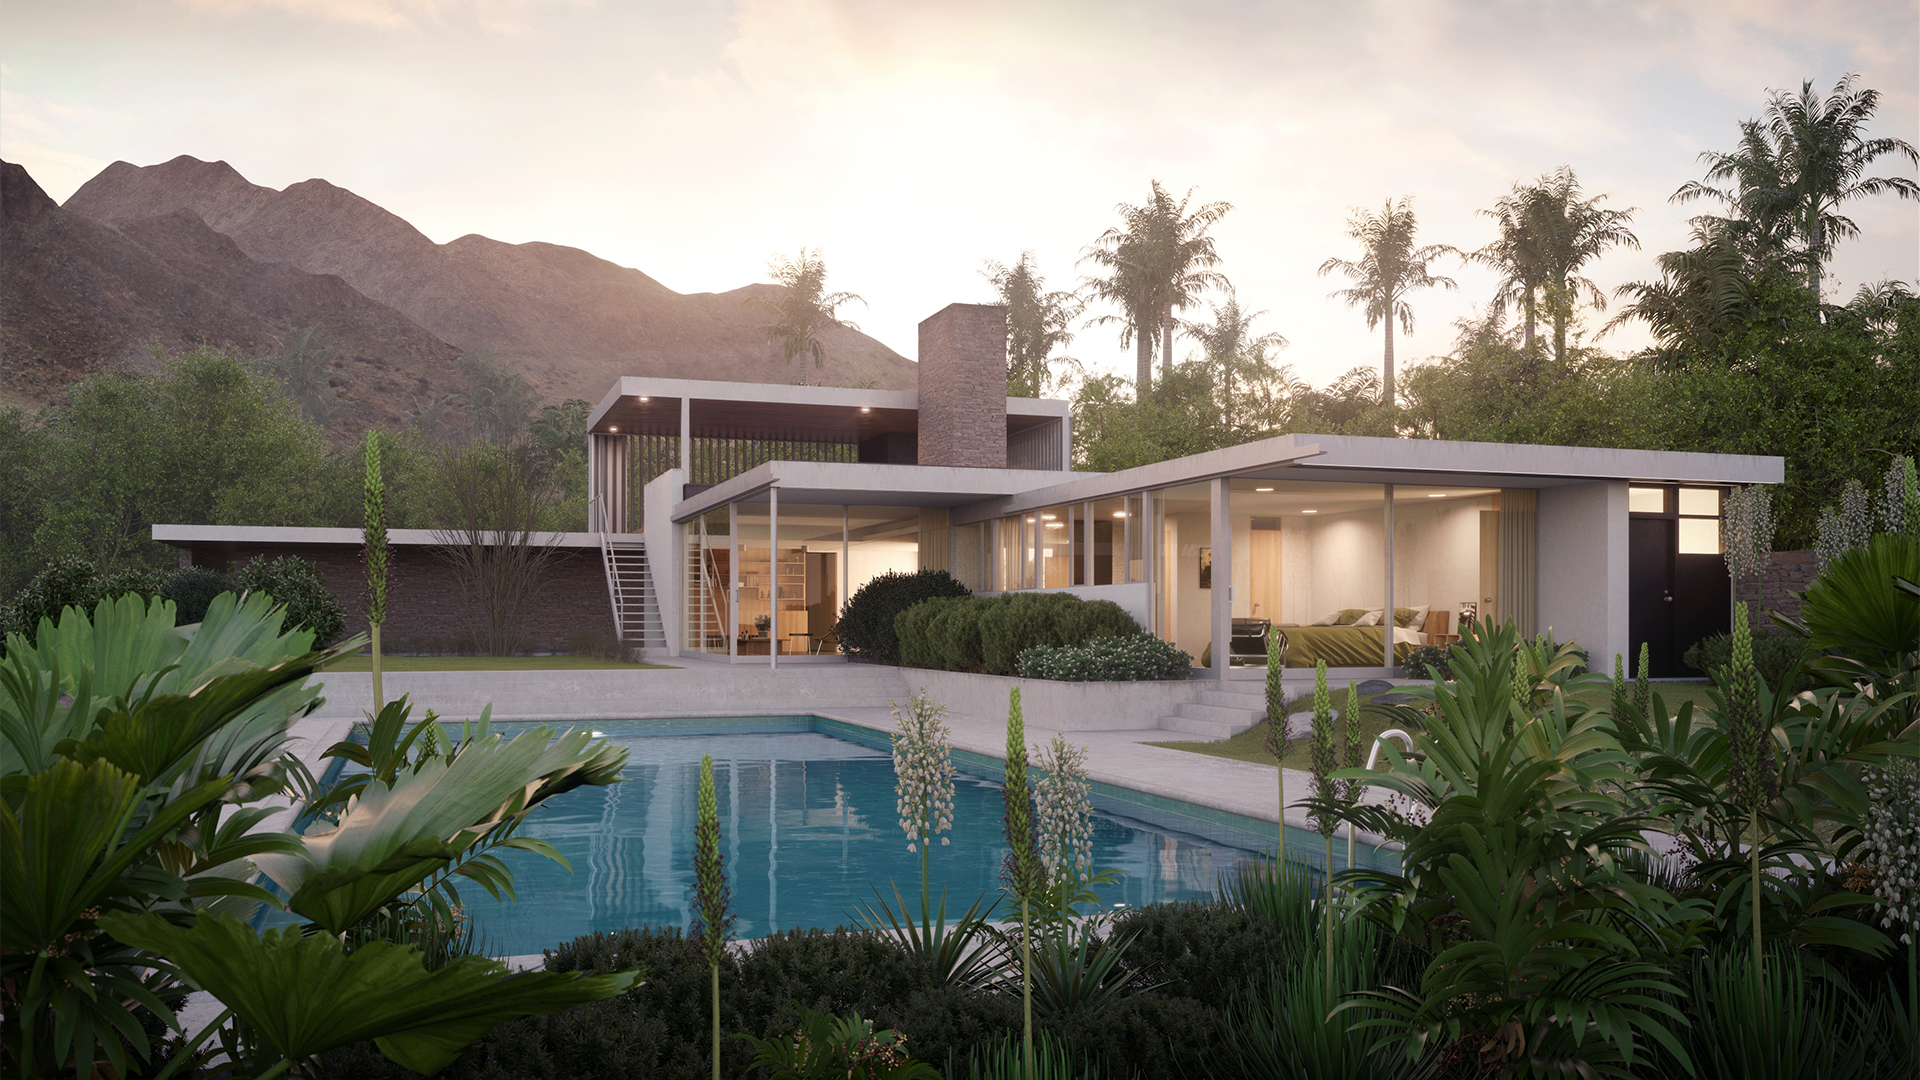
\includegraphics[width=\textwidth,height=\textheight,keepaspectratio]{../images/1_introduction/Laubwerk-Kit-12_Bauclassroom-Exterior}
  \caption{An example of a complex scene created by Laubwerk Plants Kits}
  \label{fig:intro_complexScene}
\end{figure}

After a scene is created and rendered, all the hard work invested by the artist 
is stored, waiting for a possible future use. However, should the artist choose 
to change renderers, the scene file they created so diligently would have to be 
rewritten and/or heavily modified.

Converting a scene file from one renderer format to another is very difficult 
and time consuming. Aside from adapting material and light properties - which 
can be hard since sometimes renderers don't provide the same features -, the 3D 
object formats supported may not be the same. For instance, \textit{Mitsuba} 
supports the Object File Wavefront 3D (.obj) format while \textit{PBRT} does 
not.

\section{Using PBR on Research}

Currently, PB rendering is currently the only practical solution for simulating 
global illumination effects in complex environments.

Due to its high computational cost, several techniques have been introduced to 
reduce rendering time through improved sampling~\cite{Heck2013, Pilleboue:2015} 
and reconstruction strategies~\cite{Sen2012, Rousselle2013, Kalantari2015, 
Bitterli2016}. When developing such new techniques, researchers often implement 
them on top of existing rendering systems as a way of leveraging available 
infrastructure to perform functions (\eg, ray-traversal acceleration, 
ray-primitive intersections, etc.) that are orthogonal to the proposed methods.

Unfortunately, the various rendering systems use proprietary scene description 
formats. While modeling visually-pleasing scenes requires significant artistic 
skills, manual conversion between proprietary formats requires knowledge of the 
specific formats and tend to be extremely time consuming (up to several days per 
scene~\cite{tungsten}). 

Thus, by selecting a given rendering system one is often constrained to test and 
demonstrate the proposed techniques on the limited set of test scenes available 
for that renderer. This apparently simple limitation has profound implications, 
as it constrains a direct comparison between Monte Carlo (MC) rendering 
techniques that have been implemented using different rendering systems. In this 
case, one often has to compare the quality of algorithms using disjoint sets of 
scenes, which, is not the ideal case.  

% maybe add more people complaining

\section{Project Definition}

We present {\it a system for automatic conversion among scene file formats used 
by PBR systems}. 
Our solution intends to expand the repertoire of scenes available for 
testing, validation, and benchmarking of PB rendering algorithms.  
Currently, our system handles conversions among PBRT v3~\cite{PBRT:v3}, 
Mitsuba~\cite{mitsuba}, and LuxRender~\cite{luxrender}, which are three of the 
most popular physically-based renderers. Extending it to support 
additional renderes is straightforward. Our solution (discussed in 
Section~\ref{sec:systemarch}) consists of {\it importing} any source scene 
description into a canonical representation, which can then be {\it exported} to 
other scene formats. 
%By specializing the import and export classes to the various formats, our system can convert among arbitrary scene file formats.     %
Figure~\ref{fig:teaser} illustrates the use of our system to perform automatic 
conversion of a scene represented in the PBRT v3 format. 
%The image shown on the left is the PBRT v3 rendering. 
The images at the center and on the right show, respectively, the renderings 
produced by Mitsuba and by LuxRender, from converted scenes files. Note the 
correct representation of the 
%scene elements that include multiple 
various materials (glass, plastic, and metal).

Our work does not introduce a new physically-based rendering technique per se. 
Instead, it falls in the area of {\it meta-research} systems, which are systems 
designed to facilitate and improve the research process. Meta-research systems 
are quite common in computer graphics and computer vision~\cite{MiddleburyStereo, 
MiddleburyFlow, AlphaMatting, VideoMatting}, where they have led to significant 
progress in these fields. 
%In a work particularly relevant to us,  
Recently, Santos et al.~\cite{Santos:2018:FBKSD} introduced a framework for 
developing and benchmarking MC sampling and denoising algorithms. This is 
achieved by providing an API the decouples the developed techniques from the 
used rendering system. While it allows a technique to be tested on any rendering 
system that supports the proposed API, each rendering system is still 
constrained to a limited set of test scenes. Our system is orthogonal to and 
complements the API described in~\cite{Santos:2018:FBKSD}, lending to full 
orthogonality, among algorithms, rendering systems, and scene files.
%by allowing an MC technique to be tested on any combination of rendering systems and scene files. 
%The system is also available for download~\cite{sceneConverter}.    

The {\bf contributions} of our work include:
\begin{itemize}
	\item A system for automatic conversion among scene file formats used by 
Monte Carlo physically-based rendering systems (Section~\ref{sec:systemarch}).
	It enables algorithms implemented on different rendering systems to be 
tested on similar scene descriptions, giving developers and end user a better 
assessment of the strengths and limitations of MC rendering techniques;
	\item A mechanism for achieving  orthogonality among MC rendering 
algorithms, rendering systems, and scene files (Section~\ref{sec:systemarch}). 
This is achieved in combination with the API provided 
in~\cite{Santos:2018:FBKSD}. 
\end{itemize}


<TODO>
